% ---- FHIRTrustBench evidence map (generated by results/scripts/make_evidence_map.py; locked 2026-10-26 data) ----
% Preamble: \usepackage{tikz}, \usepackage{pifont}
\definecolor{ftbS0}{HTML}{A8443A}\definecolor{ftbS1}{HTML}{D06E45}\definecolor{ftbS2}{HTML}{E9A05A}
\definecolor{ftbS3}{HTML}{F2C674}\definecolor{ftbS4}{HTML}{F8E6AE}\definecolor{ftbSNA}{HTML}{FFFFFF}
\definecolor{ftbSInk}{HTML}{2E2E2E}\definecolor{ftbSRule}{HTML}{B8B8B8}
\begin{figure}[t]
\centering
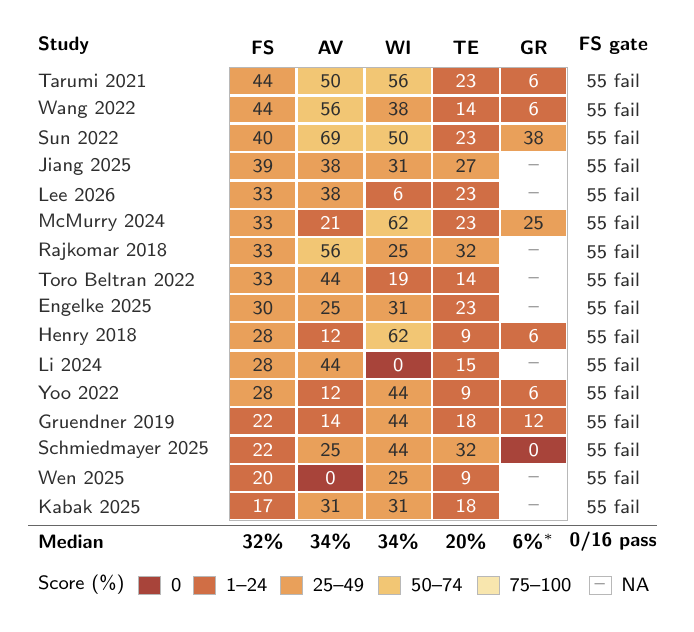
\begin{tikzpicture}[x=1cm,y=1cm,font=\scriptsize\sffamily]
\node[anchor=south west,font=\scriptsize\sffamily\bfseries] at (0,0.04) {Study};
\node[anchor=south,font=\scriptsize\sffamily\bfseries] at (2.98,0.04) {FS};
\node[anchor=south,font=\scriptsize\sffamily\bfseries] at (3.84,0.04) {AV};
\node[anchor=south,font=\scriptsize\sffamily\bfseries] at (4.70,0.04) {WI};
\node[anchor=south,font=\scriptsize\sffamily\bfseries] at (5.56,0.04) {TE};
\node[anchor=south,font=\scriptsize\sffamily\bfseries] at (6.42,0.04) {GR};
\node[anchor=south,font=\scriptsize\sffamily\bfseries] at (7.43,0.04) {FS gate};
\node[anchor=west,text=ftbSInk] at (0,-0.18) {Tarumi 2021};
\fill[ftbS2] (2.55,-0.36) rectangle (3.41,-0.00);
\node[text=ftbSInk] at (2.98,-0.18) {44};
\fill[ftbS3] (3.41,-0.36) rectangle (4.27,-0.00);
\node[text=ftbSInk] at (3.84,-0.18) {50};
\fill[ftbS3] (4.27,-0.36) rectangle (5.13,-0.00);
\node[text=ftbSInk] at (4.70,-0.18) {56};
\fill[ftbS1] (5.13,-0.36) rectangle (5.99,-0.00);
\node[text=white] at (5.56,-0.18) {23};
\fill[ftbS1] (5.99,-0.36) rectangle (6.85,-0.00);
\node[text=white] at (6.42,-0.18) {6};
\node[text=ftbSInk] at (7.43,-0.18) {\ding{55}~fail};
\node[anchor=west,text=ftbSInk] at (0,-0.54) {Wang 2022};
\fill[ftbS2] (2.55,-0.72) rectangle (3.41,-0.36);
\node[text=ftbSInk] at (2.98,-0.54) {44};
\fill[ftbS3] (3.41,-0.72) rectangle (4.27,-0.36);
\node[text=ftbSInk] at (3.84,-0.54) {56};
\fill[ftbS2] (4.27,-0.72) rectangle (5.13,-0.36);
\node[text=ftbSInk] at (4.70,-0.54) {38};
\fill[ftbS1] (5.13,-0.72) rectangle (5.99,-0.36);
\node[text=white] at (5.56,-0.54) {14};
\fill[ftbS1] (5.99,-0.72) rectangle (6.85,-0.36);
\node[text=white] at (6.42,-0.54) {6};
\node[text=ftbSInk] at (7.43,-0.54) {\ding{55}~fail};
\node[anchor=west,text=ftbSInk] at (0,-0.90) {Sun 2022};
\fill[ftbS2] (2.55,-1.08) rectangle (3.41,-0.72);
\node[text=ftbSInk] at (2.98,-0.90) {40};
\fill[ftbS3] (3.41,-1.08) rectangle (4.27,-0.72);
\node[text=ftbSInk] at (3.84,-0.90) {69};
\fill[ftbS3] (4.27,-1.08) rectangle (5.13,-0.72);
\node[text=ftbSInk] at (4.70,-0.90) {50};
\fill[ftbS1] (5.13,-1.08) rectangle (5.99,-0.72);
\node[text=white] at (5.56,-0.90) {23};
\fill[ftbS2] (5.99,-1.08) rectangle (6.85,-0.72);
\node[text=ftbSInk] at (6.42,-0.90) {38};
\node[text=ftbSInk] at (7.43,-0.90) {\ding{55}~fail};
\node[anchor=west,text=ftbSInk] at (0,-1.26) {Jiang 2025};
\fill[ftbS2] (2.55,-1.44) rectangle (3.41,-1.08);
\node[text=ftbSInk] at (2.98,-1.26) {39};
\fill[ftbS2] (3.41,-1.44) rectangle (4.27,-1.08);
\node[text=ftbSInk] at (3.84,-1.26) {38};
\fill[ftbS2] (4.27,-1.44) rectangle (5.13,-1.08);
\node[text=ftbSInk] at (4.70,-1.26) {31};
\fill[ftbS2] (5.13,-1.44) rectangle (5.99,-1.08);
\node[text=ftbSInk] at (5.56,-1.26) {27};
\fill[ftbSNA] (5.99,-1.44) rectangle (6.85,-1.08);
\node[text=black!40] at (6.42,-1.26) {--};
\node[text=ftbSInk] at (7.43,-1.26) {\ding{55}~fail};
\node[anchor=west,text=ftbSInk] at (0,-1.62) {Lee 2026};
\fill[ftbS2] (2.55,-1.80) rectangle (3.41,-1.44);
\node[text=ftbSInk] at (2.98,-1.62) {33};
\fill[ftbS2] (3.41,-1.80) rectangle (4.27,-1.44);
\node[text=ftbSInk] at (3.84,-1.62) {38};
\fill[ftbS1] (4.27,-1.80) rectangle (5.13,-1.44);
\node[text=white] at (4.70,-1.62) {6};
\fill[ftbS1] (5.13,-1.80) rectangle (5.99,-1.44);
\node[text=white] at (5.56,-1.62) {23};
\fill[ftbSNA] (5.99,-1.80) rectangle (6.85,-1.44);
\node[text=black!40] at (6.42,-1.62) {--};
\node[text=ftbSInk] at (7.43,-1.62) {\ding{55}~fail};
\node[anchor=west,text=ftbSInk] at (0,-1.98) {McMurry 2024};
\fill[ftbS2] (2.55,-2.16) rectangle (3.41,-1.80);
\node[text=ftbSInk] at (2.98,-1.98) {33};
\fill[ftbS1] (3.41,-2.16) rectangle (4.27,-1.80);
\node[text=white] at (3.84,-1.98) {21};
\fill[ftbS3] (4.27,-2.16) rectangle (5.13,-1.80);
\node[text=ftbSInk] at (4.70,-1.98) {62};
\fill[ftbS1] (5.13,-2.16) rectangle (5.99,-1.80);
\node[text=white] at (5.56,-1.98) {23};
\fill[ftbS2] (5.99,-2.16) rectangle (6.85,-1.80);
\node[text=ftbSInk] at (6.42,-1.98) {25};
\node[text=ftbSInk] at (7.43,-1.98) {\ding{55}~fail};
\node[anchor=west,text=ftbSInk] at (0,-2.34) {Rajkomar 2018};
\fill[ftbS2] (2.55,-2.52) rectangle (3.41,-2.16);
\node[text=ftbSInk] at (2.98,-2.34) {33};
\fill[ftbS3] (3.41,-2.52) rectangle (4.27,-2.16);
\node[text=ftbSInk] at (3.84,-2.34) {56};
\fill[ftbS2] (4.27,-2.52) rectangle (5.13,-2.16);
\node[text=ftbSInk] at (4.70,-2.34) {25};
\fill[ftbS2] (5.13,-2.52) rectangle (5.99,-2.16);
\node[text=ftbSInk] at (5.56,-2.34) {32};
\fill[ftbSNA] (5.99,-2.52) rectangle (6.85,-2.16);
\node[text=black!40] at (6.42,-2.34) {--};
\node[text=ftbSInk] at (7.43,-2.34) {\ding{55}~fail};
\node[anchor=west,text=ftbSInk] at (0,-2.70) {Toro Beltran 2022};
\fill[ftbS2] (2.55,-2.88) rectangle (3.41,-2.52);
\node[text=ftbSInk] at (2.98,-2.70) {33};
\fill[ftbS2] (3.41,-2.88) rectangle (4.27,-2.52);
\node[text=ftbSInk] at (3.84,-2.70) {44};
\fill[ftbS1] (4.27,-2.88) rectangle (5.13,-2.52);
\node[text=white] at (4.70,-2.70) {19};
\fill[ftbS1] (5.13,-2.88) rectangle (5.99,-2.52);
\node[text=white] at (5.56,-2.70) {14};
\fill[ftbSNA] (5.99,-2.88) rectangle (6.85,-2.52);
\node[text=black!40] at (6.42,-2.70) {--};
\node[text=ftbSInk] at (7.43,-2.70) {\ding{55}~fail};
\node[anchor=west,text=ftbSInk] at (0,-3.06) {Engelke 2025};
\fill[ftbS2] (2.55,-3.24) rectangle (3.41,-2.88);
\node[text=ftbSInk] at (2.98,-3.06) {30};
\fill[ftbS2] (3.41,-3.24) rectangle (4.27,-2.88);
\node[text=ftbSInk] at (3.84,-3.06) {25};
\fill[ftbS2] (4.27,-3.24) rectangle (5.13,-2.88);
\node[text=ftbSInk] at (4.70,-3.06) {31};
\fill[ftbS1] (5.13,-3.24) rectangle (5.99,-2.88);
\node[text=white] at (5.56,-3.06) {23};
\fill[ftbSNA] (5.99,-3.24) rectangle (6.85,-2.88);
\node[text=black!40] at (6.42,-3.06) {--};
\node[text=ftbSInk] at (7.43,-3.06) {\ding{55}~fail};
\node[anchor=west,text=ftbSInk] at (0,-3.42) {Henry 2018};
\fill[ftbS2] (2.55,-3.60) rectangle (3.41,-3.24);
\node[text=ftbSInk] at (2.98,-3.42) {28};
\fill[ftbS1] (3.41,-3.60) rectangle (4.27,-3.24);
\node[text=white] at (3.84,-3.42) {12};
\fill[ftbS3] (4.27,-3.60) rectangle (5.13,-3.24);
\node[text=ftbSInk] at (4.70,-3.42) {62};
\fill[ftbS1] (5.13,-3.60) rectangle (5.99,-3.24);
\node[text=white] at (5.56,-3.42) {9};
\fill[ftbS1] (5.99,-3.60) rectangle (6.85,-3.24);
\node[text=white] at (6.42,-3.42) {6};
\node[text=ftbSInk] at (7.43,-3.42) {\ding{55}~fail};
\node[anchor=west,text=ftbSInk] at (0,-3.78) {Li 2024};
\fill[ftbS2] (2.55,-3.96) rectangle (3.41,-3.60);
\node[text=ftbSInk] at (2.98,-3.78) {28};
\fill[ftbS2] (3.41,-3.96) rectangle (4.27,-3.60);
\node[text=ftbSInk] at (3.84,-3.78) {44};
\fill[ftbS0] (4.27,-3.96) rectangle (5.13,-3.60);
\node[text=white] at (4.70,-3.78) {0};
\fill[ftbS1] (5.13,-3.96) rectangle (5.99,-3.60);
\node[text=white] at (5.56,-3.78) {15};
\fill[ftbSNA] (5.99,-3.96) rectangle (6.85,-3.60);
\node[text=black!40] at (6.42,-3.78) {--};
\node[text=ftbSInk] at (7.43,-3.78) {\ding{55}~fail};
\node[anchor=west,text=ftbSInk] at (0,-4.14) {Yoo 2022};
\fill[ftbS2] (2.55,-4.32) rectangle (3.41,-3.96);
\node[text=ftbSInk] at (2.98,-4.14) {28};
\fill[ftbS1] (3.41,-4.32) rectangle (4.27,-3.96);
\node[text=white] at (3.84,-4.14) {12};
\fill[ftbS2] (4.27,-4.32) rectangle (5.13,-3.96);
\node[text=ftbSInk] at (4.70,-4.14) {44};
\fill[ftbS1] (5.13,-4.32) rectangle (5.99,-3.96);
\node[text=white] at (5.56,-4.14) {9};
\fill[ftbS1] (5.99,-4.32) rectangle (6.85,-3.96);
\node[text=white] at (6.42,-4.14) {6};
\node[text=ftbSInk] at (7.43,-4.14) {\ding{55}~fail};
\node[anchor=west,text=ftbSInk] at (0,-4.50) {Gruendner 2019};
\fill[ftbS1] (2.55,-4.68) rectangle (3.41,-4.32);
\node[text=white] at (2.98,-4.50) {22};
\fill[ftbS1] (3.41,-4.68) rectangle (4.27,-4.32);
\node[text=white] at (3.84,-4.50) {14};
\fill[ftbS2] (4.27,-4.68) rectangle (5.13,-4.32);
\node[text=ftbSInk] at (4.70,-4.50) {44};
\fill[ftbS1] (5.13,-4.68) rectangle (5.99,-4.32);
\node[text=white] at (5.56,-4.50) {18};
\fill[ftbS1] (5.99,-4.68) rectangle (6.85,-4.32);
\node[text=white] at (6.42,-4.50) {12};
\node[text=ftbSInk] at (7.43,-4.50) {\ding{55}~fail};
\node[anchor=west,text=ftbSInk] at (0,-4.86) {Schmiedmayer 2025};
\fill[ftbS1] (2.55,-5.04) rectangle (3.41,-4.68);
\node[text=white] at (2.98,-4.86) {22};
\fill[ftbS2] (3.41,-5.04) rectangle (4.27,-4.68);
\node[text=ftbSInk] at (3.84,-4.86) {25};
\fill[ftbS2] (4.27,-5.04) rectangle (5.13,-4.68);
\node[text=ftbSInk] at (4.70,-4.86) {44};
\fill[ftbS2] (5.13,-5.04) rectangle (5.99,-4.68);
\node[text=ftbSInk] at (5.56,-4.86) {32};
\fill[ftbS0] (5.99,-5.04) rectangle (6.85,-4.68);
\node[text=white] at (6.42,-4.86) {0};
\node[text=ftbSInk] at (7.43,-4.86) {\ding{55}~fail};
\node[anchor=west,text=ftbSInk] at (0,-5.22) {Wen 2025};
\fill[ftbS1] (2.55,-5.40) rectangle (3.41,-5.04);
\node[text=white] at (2.98,-5.22) {20};
\fill[ftbS0] (3.41,-5.40) rectangle (4.27,-5.04);
\node[text=white] at (3.84,-5.22) {0};
\fill[ftbS2] (4.27,-5.40) rectangle (5.13,-5.04);
\node[text=ftbSInk] at (4.70,-5.22) {25};
\fill[ftbS1] (5.13,-5.40) rectangle (5.99,-5.04);
\node[text=white] at (5.56,-5.22) {9};
\fill[ftbSNA] (5.99,-5.40) rectangle (6.85,-5.04);
\node[text=black!40] at (6.42,-5.22) {--};
\node[text=ftbSInk] at (7.43,-5.22) {\ding{55}~fail};
\node[anchor=west,text=ftbSInk] at (0,-5.58) {Kabak 2025};
\fill[ftbS1] (2.55,-5.76) rectangle (3.41,-5.40);
\node[text=white] at (2.98,-5.58) {17};
\fill[ftbS2] (3.41,-5.76) rectangle (4.27,-5.40);
\node[text=ftbSInk] at (3.84,-5.58) {31};
\fill[ftbS2] (4.27,-5.76) rectangle (5.13,-5.40);
\node[text=ftbSInk] at (4.70,-5.58) {31};
\fill[ftbS1] (5.13,-5.76) rectangle (5.99,-5.40);
\node[text=white] at (5.56,-5.58) {18};
\fill[ftbSNA] (5.99,-5.76) rectangle (6.85,-5.40);
\node[text=black!40] at (6.42,-5.58) {--};
\node[text=ftbSInk] at (7.43,-5.58) {\ding{55}~fail};
\draw[white,line width=0.9pt] (2.55,-0.00) -- (6.85,-0.00);
\draw[white,line width=0.9pt] (2.55,-0.36) -- (6.85,-0.36);
\draw[white,line width=0.9pt] (2.55,-0.72) -- (6.85,-0.72);
\draw[white,line width=0.9pt] (2.55,-1.08) -- (6.85,-1.08);
\draw[white,line width=0.9pt] (2.55,-1.44) -- (6.85,-1.44);
\draw[white,line width=0.9pt] (2.55,-1.80) -- (6.85,-1.80);
\draw[white,line width=0.9pt] (2.55,-2.16) -- (6.85,-2.16);
\draw[white,line width=0.9pt] (2.55,-2.52) -- (6.85,-2.52);
\draw[white,line width=0.9pt] (2.55,-2.88) -- (6.85,-2.88);
\draw[white,line width=0.9pt] (2.55,-3.24) -- (6.85,-3.24);
\draw[white,line width=0.9pt] (2.55,-3.60) -- (6.85,-3.60);
\draw[white,line width=0.9pt] (2.55,-3.96) -- (6.85,-3.96);
\draw[white,line width=0.9pt] (2.55,-4.32) -- (6.85,-4.32);
\draw[white,line width=0.9pt] (2.55,-4.68) -- (6.85,-4.68);
\draw[white,line width=0.9pt] (2.55,-5.04) -- (6.85,-5.04);
\draw[white,line width=0.9pt] (2.55,-5.40) -- (6.85,-5.40);
\draw[white,line width=0.9pt] (2.55,-5.76) -- (6.85,-5.76);
\draw[white,line width=0.9pt] (2.55,0) -- (2.55,-5.76);
\draw[white,line width=0.9pt] (3.41,0) -- (3.41,-5.76);
\draw[white,line width=0.9pt] (4.27,0) -- (4.27,-5.76);
\draw[white,line width=0.9pt] (5.13,0) -- (5.13,-5.76);
\draw[white,line width=0.9pt] (5.99,0) -- (5.99,-5.76);
\draw[white,line width=0.9pt] (6.85,0) -- (6.85,-5.76);
\draw[ftbSRule,line width=0.3pt] (2.55,0) rectangle (6.85,-5.76);
\draw[black!60,line width=0.4pt] (0,-5.82) -- (7.98,-5.82);
\node[anchor=west,font=\scriptsize\sffamily\bfseries] at (0,-6.03) {Median};
\node[font=\scriptsize\sffamily\bfseries] at (2.98,-6.03) {32\%};
\node[font=\scriptsize\sffamily\bfseries] at (3.84,-6.03) {34\%};
\node[font=\scriptsize\sffamily\bfseries] at (4.70,-6.03) {34\%};
\node[font=\scriptsize\sffamily\bfseries] at (5.56,-6.03) {20\%};
\node[font=\scriptsize\sffamily\bfseries] at (6.42,-6.03) {6\%$^{*}$};
\node[font=\scriptsize\sffamily\bfseries] at (7.43,-6.03) {0/16 pass};
\node[anchor=west] at (0,-6.58) {Score (\%)};
\fill[ftbS0] (1.40,-6.69) rectangle (1.68,-6.47);
\draw[ftbSRule,line width=0.2pt] (1.40,-6.69) rectangle (1.68,-6.47);
\node[anchor=west] at (1.69,-6.58) {0};
\fill[ftbS1] (2.10,-6.69) rectangle (2.38,-6.47);
\draw[ftbSRule,line width=0.2pt] (2.10,-6.69) rectangle (2.38,-6.47);
\node[anchor=west] at (2.39,-6.58) {1--24};
\fill[ftbS2] (3.20,-6.69) rectangle (3.48,-6.47);
\draw[ftbSRule,line width=0.2pt] (3.20,-6.69) rectangle (3.48,-6.47);
\node[anchor=west] at (3.49,-6.58) {25--49};
\fill[ftbS3] (4.45,-6.69) rectangle (4.73,-6.47);
\draw[ftbSRule,line width=0.2pt] (4.45,-6.69) rectangle (4.73,-6.47);
\node[anchor=west] at (4.74,-6.58) {50--74};
\fill[ftbS4] (5.70,-6.69) rectangle (5.98,-6.47);
\draw[ftbSRule,line width=0.2pt] (5.70,-6.69) rectangle (5.98,-6.47);
\node[anchor=west] at (5.99,-6.58) {75--100};
\draw[ftbSRule,line width=0.2pt] (7.12,-6.69) rectangle (7.40,-6.47);
\node[text=black!40] at (7.26,-6.58) {--};
\node[anchor=west] at (7.41,-6.58) {NA};
\end{tikzpicture}
\caption{FHIRTrustBench applied to 16 published FHIR-integrated clinical AI systems, using the adjudicated codes. Each cell is the share of attainable points on the applicable sub-criteria of a dimension (Met = 2, Partial = 1, not met or not reported = 0); rows are sorted by FHIR specificity. No system passes the FHIR-specificity gate (FS1 and FS3 at least Partial and FS $\geq$ 50\%); the highest FS score is 44\%. -- = fewer than three applicable sub-criteria; $^{*}$ median over the eight studies with a defined GR score.}
\Description{A heatmap with 16 studies as rows and the five FHIRTrustBench dimensions as columns. Most cells fall in the 0 to 49 percent bands, governance is undefined for half of the studies, and every study is marked as failing the FHIR-specificity gate.}
\label{fig:evidencemap}
\end{figure}
